\documentclass[../../topologia_algebraica]{subfiles}
\begin{document}
\section{Producto cu\~na}

A lo largo de las siguientes tres secciones voy a desarrollar herramienta topol\'ogica para poder
estudiar a fondo la relaci\'on
\[
  \pi_n(X,x_0):=\Big[(\Sn^n,1),(X,x_0)\Big]
\]
y c\'omo usarlo para relacionar los diferentes grupos fundamentales de un espacio basado. La primera
construcci\'on es el producto cu\~na:

Sea $\{(X_j,x_j)\}_{j\in J}$ una familia de espacios basados, $\sqcup_{j}(X_j,x_j)$ su uni\'on disjunta
e identifico todos los puntos base en uno s\'olo. M\'as precisamente defino
$B=\{x_j\}_{j\in J}$, el conjunto de todos los puntos bases y hago cociente sobre $B$ (ie. identifico
a todos los elementos en $B$ y a los dem\'as los identifico s\'olo con ellos mismos). As\'i si
define el producto cu\~na:
\[
  \bigvee_{j\in J}(X_j,x_j):= \frac{\bigsqcup(X_j,x_j)}{\{x_j\}}
\]
con la topolog\'ia cociente.

\begin{lema}\label{lem:cuna_coproducto}
  El producto cu\~na en $\mathbf{Top}_*$ es un coproducto, es decir para cualquier familia
  $\{(X_j,x_j)\}_{j\in J}$ de espacios basados existen morfismos
  $\{\mu_i:(X_i,x_i)\ra \vee (X_j,x_j)\}_{j\in J}$ tales que cumplen la siguiente propiedad
  universal: Si $(Y,y_0)$ es cualquier espacio basado junto con morfismos
  $\{f_i:(X_i,x_i)\ra (Y,y_0)\}_{i\in J}$ entonces existe un \'unico morfismo
  $\theta:\vee(X_j,x_j)\ra (Y,y_0)$ que hace el siguiente
  diagrama conmutar:
  \begin{equation}\label{cd:cuna_coproducto}
    \begin{tikzcd}
      \bigvee(X_j,x_j) \arrow[rr,dashed,"\theta"] & & (Y,y_0) \\
      & (X_i,x_i) \arrow[ul,"\mu_i"] \arrow[ur,"f_i"'] &
    \end{tikzcd}
  \end{equation}
\end{lema}
\begin{proof}
  Primero exhibo los morfismos $\mu_i:(X_i,x_i)\ra\vee(X_j,x_j)$: para toda $i\in J$, existe una
  inclusi\'on natural:
  \[
    u_i:(X_i,x_i) \lra \bigsqcup_{j\in J} (X_j,x_j)
  \]
  que hace $x\mapsto x\in\sqcup(X_j,x_j)$. Si compongo esta inclusi\'on con la identificaci\'on
  natural $\nu:\sqcup(X_j,x_j)\epi\vee(X_j,x_j)$, puedo definir $\mu_i:=\nu\circ u_i$. Afirmo
  que $\vee(X_j,x_j)$ junto con $\{\mu_i:(X_i,x_i)\ra\vee(X_j,x_j)\}$ es un coproducto.

  Sea $(Y,y_0)$ un espacio basado con morfismos $\{f_i:(X_i,x_i)\ra (Y,y_0)\}_{i\in J}$.
  Puedo definir de manera natural la funci\'on: 
  \[
    \sqcup f_j:\bigsqcup_{j\in J}(X_j,x_j)\lra (Y,y_0) \quad\text{con}\quad
    (\sqcup f_j(x))=f_i(x) \;\;\text{si}\;\; x\in X_i.
  \]
  Como la uni\'on es disjunta, $\sqcup f_j$ est\'a bien definida y es continua (porque cada $f_j$
  lo es). Observa que por definici\'on $f_i=\sqcup f_j\circ u_i$ donde $u_i$ es la inclusi\'on
  natural de $(X_i,x_i)$ en $\sqcup (X_i,x_i)$.

  Adem\'as, es una funci\'on basada porque $\sqcup f_j(x_i)=f_i(x_i)=y_0$ para toda $i\in J$.
  Esta \'ultima igualdad implica que $(\sqcup f_j)[B]=\{y_0\}$ y as\'i $\sqcup f_j$ se factoriza a
  trav\'es de $\vee(X_j,x_j)$; a esta nueva funci\'on (continua de espacios basados) la llamo
  $\vee f_j$:
  \[
    \begin{tikzcd}
      \bigsqcup (X_j,x_j) \arrow[r,"\sqcup f_j"] \arrow[d,twoheadrightarrow,"\nu"'] & (Y,y_0) \\
      \bigvee (X_j,x_j) \arrow[ur,dashed,"\vee f_j"']
    \end{tikzcd}
    \qquad \sqcup f_j=\vee f_j \circ \nu
  \]

  Ahora s\'olo falta ver que $\theta=\vee f_j$ satisface el diagrama conmutativo
  (\ref{cd:cuna_coproducto}), es decir que $f_i=\vee f_j\circ \mu_i$. Esto se sigue inmediatamente
  de todas las definiciones que he dado y el diagrama conmutativo anterior:
  \[
    \vee f_j \circ \mu_i =\vee f_j \circ (\nu \circ u_i)=(\vee f_j \circ \nu) \circ u_i=
    \sqcup f_j \circ u_i=f_i.
  \]
  Observa que si $\star\in\vee (X_j,x_j)$ es su punto base natural, entonces para
  $x_i\in(X_i,x_i)$ en la preimagen bajo (cualquier) $\mu_i$ tenemos que
  $\vee f_j(\star)=\vee f_j(\mu_i(x_i))=
  f_i(x_i)=y_0$. Entonces $\vee f_j$ es un morfismo en $\mathbf{Top}_*$.

  La unicidad de $\vee f_j$ se sigue de que el coproducto es un objeto inicial en una categor\'ia
  adecuada.  
\end{proof}

\begin{nota}
  Al morfismo $\vee f_j$ se le puede dar una f\'ormula: sea $[x]\in\vee(X_j,x_j)$, entonces
  $x\in\sqcup (X_j,x_j)$ y puedo asumir sin p\'erdida de generalidad que $x\in X_i$ para una
  $i\in J$. Observa que $\sqcup f_j(x)=f_i(x)\in Y$. Por construcci\'on tengo que
  \[
    \vee f_j([x])=f_i(x) \quad\text{si}\quad x\in(X_i,x_i).
  \]
\end{nota}

Antes de seguir, observa que si considero el producto cu\~na de dos espacios $(X,x_0)$ y $(Y,y_0)$
entonces hay una manera can\'onica de ver $X\vee Y$ encajado en $X\times Y$ como el conjunto
$(X\times \{y_0\})\cup(\{x_0\}\times Y)$. Ve la figura \ref{fig:cuna_encajado_en_producto}
%%%%%%%%%%%%%%%%%%%%%%%%%%%%%%%%%%%%%%%%%%%%%%%%%%%%%%%%%%%%%%%%%%%%%%%%%%%%%%%%%%%%%%% FIGURA
\begin{figure}
 \begin{minipage}{.5\textwidth}
  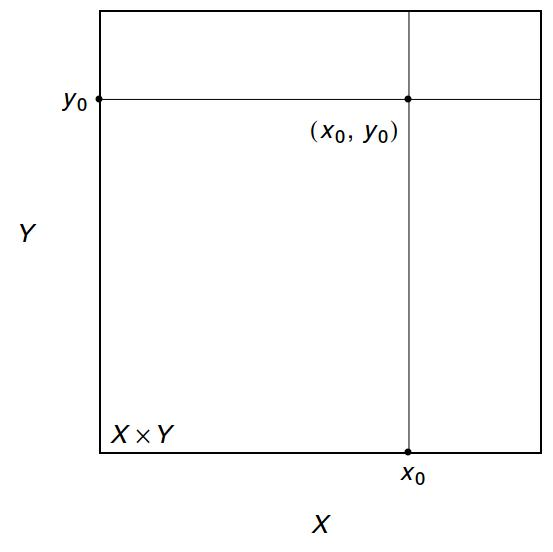
\includegraphics[scale=0.25]{cuna_encajado_en_producto}\centering
  \caption{$X\vee Y\subset X\times Y$}
  \label{fig:cuna_encajado_en_producto}
 \end{minipage}
 \begin{minipage}{.5\textwidth}
   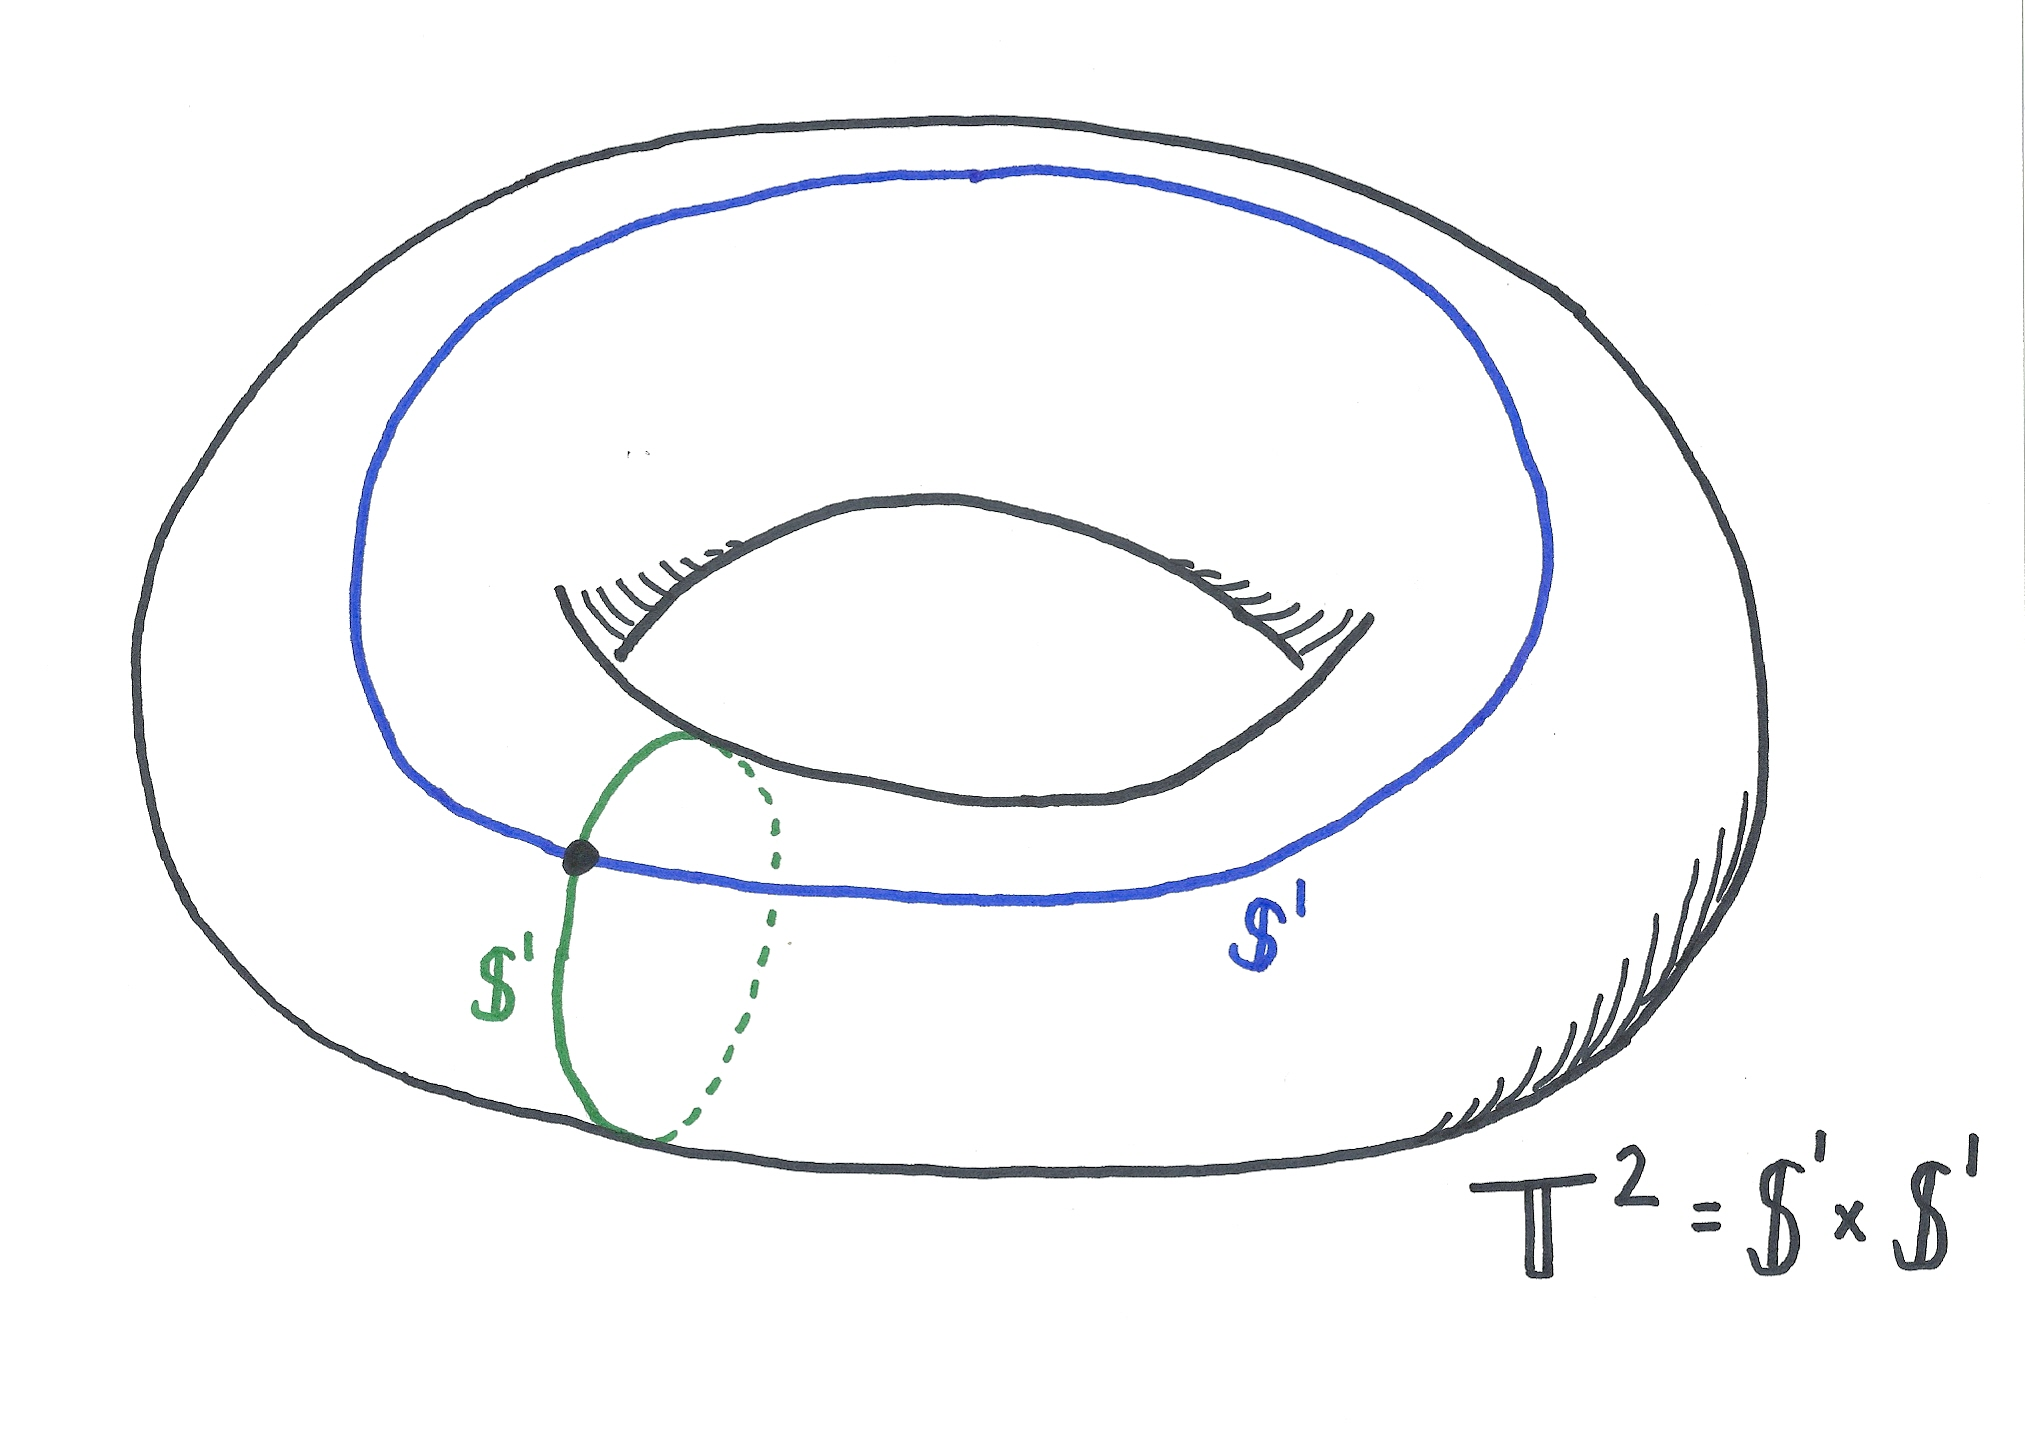
\includegraphics[scale=0.1]{cuna_de_circulos_en_toro}\centering
  \caption{$\Sn^1\vee\Sn^1\subset \TT^2$}
  \label{fig:cuna_de_circulos_en_toro}
 \end{minipage}
\end{figure}
%%%%%%%%%%%%%%%%%%%%%%%%%%%%%%%%%%%%%%%%%%%%%%%%%%%%%%%%%%%%%%%%%%%%%%%%%%%%%%%%%%%%%%%%%%%%%%
para el caso general y la figura \ref{fig:cuna_de_circulos_en_toro} para el caso particular
$\Sn^1\vee\Sn^1\subset\TT^2$.

En efecto, si denoto $V:=(X\times \{y_0\})\cup(\{x_0\}\times Y)$ y defino las siguientes dos
funciones $f_X:X\ra V$ y $f_Y:Y\ra V$ como
\[
  f_X(x)=(x,y_0) \quad\text{y}\quad f_Y(y)=(x_0,y),
\]
claramente tengo dos morfismos de espacios basados (ie. $f_X$ y $f_Y$ son continuas y basadas)
y como el producto cu\~na es un coproducto en $\mathbf{Top}_*$ existe un \'unico morfismo
$g:=f_X\vee f_Y$ de $X\vee Y$ a $V$ tal que:
\[
  g\big([z]\big)=
  \begin{cases}
    f_X(z)=(z,y_0) &\text{si}\;\; z\in X \\
    f_Y(z)=(x_0,z) &\text{si}\;\; z\in Y    
  \end{cases}
\]

Para construir el inverso, observa que $V$ se puede descomponer un una uni\'on disjunta
$V=((X-x_0)\times\{y_0\})\sqcup(\{y_0\}\times(Y-y_0))\sqcup\{(x_0,y_0)\}$. Ahora defino
la siguiente funci\'on:
\[
  h(x,y):=
  \begin{cases}
    [x] &\text{si}\;\; x\neq x_0,\; y=y_0 \\
    [y] &\text{si}\;\; x= x_0,\; y\neq y_0 \\
    \star &\text{si}\;\; x= x_0,\; y=y_0 \\
  \end{cases}
\]
donde $\star\in X\vee Y$ es el punto base can\'onico (ie $\star=[x_0]=[y_0]$). Esta funci\'on es
claramente continua porque sobre cada componente de $V$, $h$ es la restricci\'on de la funci\'on
continua $X\ra X\vee Y$, $Y\ra X\vee Y$ y la funci\'on constante $(x_0,y_0)\mapsto\star$. Claramente:
\[
  (g\circ h)(x,y)=
    \begin{cases}
    g([x])=(x,y_0) &\text{si}\;\; x\neq x_0,\; y=y_0 \\
    g([y])=(x_0,y) &\text{si}\;\; x= x_0,\; y\neq y_0 \\
    g(\star)=(x_0,y_0) &\text{si}\;\; x= x_0,\; y=y_0 \\
  \end{cases}=\Id_V
\]
y
\[
  (h\circ g)\big([z]\big)=
  \begin{cases}
    h(z,y_0)=[z] &\text{si}\;\; z\in X \\
    h(x_0,z)=[z] &\text{si}\;\; z\in Y    
  \end{cases}=\Id_{X\vee Y}.
\]

por lo tanto $X\vee Y \approx V=(X\times \{y_0\})\cup(\{x_0\}\times Y)\subset X\times Y$. Observa
que la continuidad de $g$ y $h$ requieren que $V$ tenga la topolog\'ia de subespacio de la topolog\'ia
producto en $X\times Y$.

En general, si tomamos el producto cu\~na de una familia arbitraria de espacios basados, no
necesariamente podemos encajar $\vee(X_j,x_j)$ en $\prod (X_j,x_j)$ (ie. que $\vee(X_j,x_j)$ sea
homeomorfo a su imagen). Pero no todo se pierde:

\import{\directory}{ejercicios/6}  %%%%%%%%%%%%%%%%%%%%%%%%%%%%%%%%%%%%%%%%%%%%%%%%%%%%%% EJERCICIO 6
\end{document}